
\documentclass[a4paper,11pt]{article}

% Math symbols
\usepackage{amsmath}
\usepackage{amsfonts}
\usepackage{esvect}

% Hyperlink contents page
\usepackage{hyperref}
\hypersetup{
	colorlinks,
	citecolor=black,
	filecolor=black,
	linkcolor=black,
	urlcolor=black
}

% AI files
\usepackage{graphicx}
\DeclareGraphicsRule{.ai}{pdf}{.ai}{}

% No indent on new paragraphs
\setlength{\parindent}{0mm}
\setlength{\parskip}{0.3cm}

% Alias \boldsymbol to \bb for vectors
\newcommand{\bb}{\boldsymbol}


\begin{document}

\title{Protection}
\author{Ben Anderson}
\date{\today}
\maketitle
\pagebreak

\tableofcontents
\pagebreak


\section{Protection}

\subsection{Definition}

An action by the government designed to give an artificial advantage to
domestic producers over overseas producers.

Attempts to encourage domestic production in the protected industry.


\subsection{Classification}

\textbf{Quantitive} \quad Limit the amount and distribution of an import.
Includes quotas, licenses, embargos.

\textbf{Reduce Costs} \quad Reduce costs for the domestic producer. Includes
subsidies, taxation exemptions.

\textbf{Increase Import Prices} \quad Increase the price of imported goods.
Includes tariffs.




\section{Tariffs}

\subsection{Definition}

A tax on imports through the required payment of a customs duty. A tariff has
the effect of raising the price of an imported good.


\subsection{Supply and Demand Model}

\begin{figure}
\begin{center}
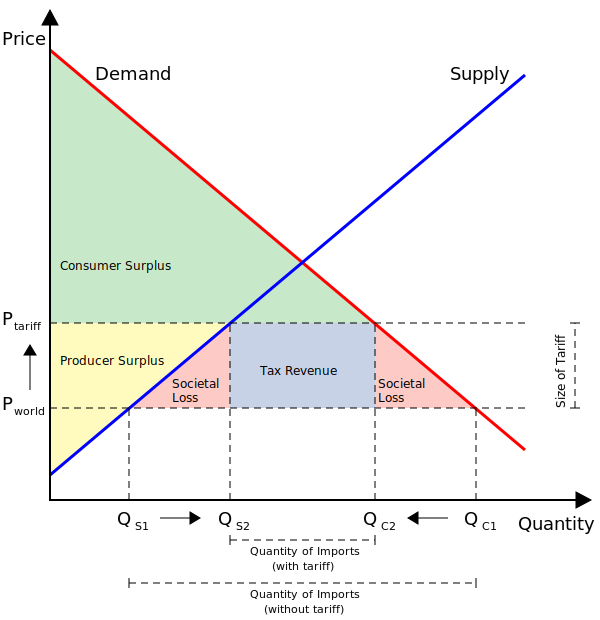
\includegraphics{tariff.ai}
\end{center}
\end{figure}

The implementation of a tariff causes:

\begin{itemize}
\item Increases the price of the good in the domestic market from the world
	price (PW) to the world price plus the price of the tarrif (PT).
\item Decreases quantity demanded from QD1 to QD2.
\item Increases quantity supplied from QS1 to QS2.
\item Decreases consumer surplus.
\item Increases producer surplus by less than the decrease in consumer surplus.
\item Increases deadweight loss.
\item Increases tax revenue.
\item Decreases total surplus and net societal welfare.
\end{itemize}


\subsection{Benefits}

\begin{description}
\item [Revenue] Allows domestic producers to raise their prices to earn
	more revenue.
\item [Competition] Allows domestic producers to compete more effectively with
	international producers and capture a larger share of the market.
\item [Jobs] Protects or creates jobs in the protected industry.
\item [Tax Revenue] Raises tax revenue for the government.
\end{description}


\subsection{Costs}

\begin{description}
\item [Consumer Prices] Consumers must pay a higher price for the product,
	reducing real income.
\item [Inefficiency] Reallocates resources from efficient industries to less
	efficient ones.
\item [Competition] Reduces competition, increasing inefficiency and costs
	(threatens growth and employment in other industries).
\item [Retaliation] Encourages retaliation from other countries (other countries
	begin to tax Australian exports because we are taxing their imports).
\item [Reliance] May result in the protected industry becoming reliant on the
	protection to survive, ultimately failing once the protection is removed.
\end{description}


\subsection{Effects}

\begin{description}
\item [Price Effect] Increases the price of the good. Increases
	inflationary pressures.
\item [Consumption Effect] Higher price causes a decrease in demand for
	the good.
\item [Protection Effect] Increases the quantity of the good produced
	domestically, decreasing the quantity of imported goods.
\item [Redistribution Effect] Decrease in consumer surplus and increase
	in producer surplus.
\item [Revenue Effect] Increases tax revenue for the government which
	they could use for other beneficial projects.
\end{description}




\section{Subsidies}

\subsection{Definition}

A payment or grant to the domestic producer by the government designed to reduce
their costs of production.


\subsection{Supply and Demand Model}

The implementation of a subsidy:

\begin{itemize}
\item No change in price of the good.
\item Shifts the domestic supply curve to the right, increasing the quantity of
	good supplied due to lower production costs for domestic producers.
\item Increases market share of domestic producers.
\item Decreases imported quantity.
\item Increases producer surplus.
\item No change in consumer surplus.
\item Increases deadweight loss reducing net societal welfare.
\end{itemize}


\subsection{Benefits}

\begin{description}
\item [Consumer Prices] Maintain lower prices for consumers, resulting in less
	consumer backlash to the introduction of a form of protection.
\item [Review] Likely subject to more regular governmental review as they are
	financed through general taxation.
\end{description}


\subsection{Costs}

\begin{description}
\item [Taxation] Higher effective taxation by the government to finance the
	subsidy.
\item [Consumption] Decreases consumption in other industries due to higher
	effective taxation.
\item [Opportunity Cost] The opportunity cost of financing the subsity,
	removing money from other potentially more worthwhile governmental services.
\end{description}




\section{Quota}

\subsection{Definition}

A quantitative restriction on the imported amounts of certain categories of
goods.

The smaller the quota, the fewer goods that may be imported, the stronger the
protection effect.


\subsection{Supply and Demand Model}

The implementation of a quota:

\begin{itemize}
\item Restricts the imported quantity of a good.
\item Creates market shortage.
\item Price of good is increased to clear the market shortage.
\item Increases the market share of domestic producers.
\item Increases producer surplus.
\item Decreases consumer surplus.
\end{itemize}


\subsection{Effects}

The same as for a tariff, except for:

\begin{description}
\item [Revenue Effect] Since there is no apparent increase in taxation,
	the government does not immediately earn a higher revenue. Instead, the
	government may charge for licenses on the imported good, still receiving
	revenue from the implementation of a quota.
\end{description}




\section{Other Forms of Protection}

\subsection{Embargo}

A complete ban on a category of imported goods.

Usually used for safety or political reasons (eg. faulty crash helmets, or
banning goods from a country run by a dictator).


\subsection{Voluntary Export Restraints}

A voluntary restriction on the exported amount of a particular good to a
particular importing country to appease them and avoid a potentially damaging
trade scenario (eg. a trade war).


\subsection{Technical Specification}

An embargo on a good that does not meet a technical requirement, eg. left hand
drive cars.


\subsection{Government Procurement Policies}

Where the government itself contracts out required services or the manufacture
of required goods to Australian firms, despite it being potentially cheaper to
import.




\section{Reasons for Protection}

\subsection{Infant Industries}

The government protects small industries that are currently inefficient, but
have the potential to be efficient given the chance to grow and achieve
economies of scale.

Protection would allow them to compete with mature overseas competition,
allowing the industry to become competitive over time.

Leads to diversification in a country's industry base. Potentially increases
exports or substitution of imports with domestically produced goods. Decreases
reliance on a few industries, making the country less susceptible to economic
swings.


\subsection{Anti-Dumping}

Dumping is when an overseas producer temporarily floods a domestic market with
an imported good sold at or below cost, which endangers the survival of the
competing local industry.

This is done to clear a surplus for the international producer, but destabilises
the local market.

Protection is used temporarily to ensure the survival of the local industry.


\subsection{Strategic Industries}

Industries considered vital to the economy (eg. banking, insurance, agriculture)
which must survive despite overseas competition.

To maintain food, water, and energy security in case of a catastrophic world
event.


\subsection{Structural Unemployment}

Minimise the effect of structural unemployment in industries severely impacted
by temporary macroeconomic events (eg. GFC) through protection, ensuring their
survival.


\subsection{Consumer Safety}

Import restrictions are placed on goods that are deemed hazardous to consumers
or the environment.


\subsection{Unrealistic Assumptions}

The comparative advantage model is based on unrealistic assumptions such as:

\begin{itemize}
\item The world consists of 2 countries producing 2 goods.
\item The countries have identical resources.
\item Resources are perfectly mobile. They can be reallocated to the production
of another good with no associated cost.
\item There are no transportation costs.
\item There are no pre-existing trade agreements or restrictions.
\end{itemize}




\section{Arguments Against Protection}

\subsection{Exports}

\begin{description}
\item [Inefficiency] Allows inefficient allocation of resources in the market
	to survive, increasing deadweight loss and reducing net societal welfare.
\item [Domestic Competition] Reduces competition, allowing inefficiencies to
	survive.
\item [Exchange Rate] Appreciates the exchange rate (reduced imports decreases
	supply of the Australian dollar), decreasing our exports' international
	competitiveness.
\item [Cost of Intermediate Goods] Increases costs for domestic producers
	previously importing a now protected intermediate good.
\item [Export Market Competition] Increases competition in our export markets
	(reduced import purchases causes international producers to sell more goods
	into markets we're trying to compete in).
\item [Spending Power] Reduces the international spending power of other
	countries (reduced purchases of their exports, decreasing their export
	income).
\end{description}


\subsection{Inflation}

\begin{itemize}
\item Increases import costs.
\item Raises production costs for firms purchasing intermediate goods.
\item Raises wage costs due to rising profits in firms.
\item Reduces competition, raising price of goods.
\end{itemize}


\subsection{Growth}

\begin{itemize}
\item Inefficient resource allocation reduces potential for economic growth.
\item Reduces incentive for firms to grow by reducing competition.
\item Reduces aggregate demand by decreasing consumption of the protected good
	(only applies for tariffs and quotas)
\end{itemize}


\subsection{Unemployment}

\begin{itemize}
\item Increases inflation, reducing real income.
\item Reduces exports, reducing firm revenue and increasing unemployment.
\end{itemize}


\subsection{Welfare}

\begin{itemize}
\item Reduces total surplus (reduced sum of consumer and producer surpluses).
\item Increases deadweight loss.
\item Reduces net welfare.
\end{itemize}

\end{document}
